\chapter{Extreme mass ratio inspirals}\label{chap:emris}
We have seen that the spiraling motions of large masses lead to the emission of gravitational waves. To be able to detect such gravitational waves buried in the noise of the detector, it is crucial to have very precise predictions of the expected waveform or signal. We will see the importance later in \fullref{ch:data-analyses} when we discuss the matched filtering technique. In this chapter we will introduce the theoretical approaches for the gravitational wave signal of an extreme mass ratio inspiral (EMRI) event under further consideration of computational cost. In the end we need to be able to create large samples of these waveforms to study the data analysis techniques and to make predictions for the LISA mission. EMRIs are mainly produced by compact objects (CO) of order $\sim 10\Msol$ that inspiral into massive black holes (MBH) of order $10^4 - 10^7 \Msol$, at least if we restrict ourselves to the events that will be observed by LISA. Depending on astrophysical models there are different expectations on the number of observed EMRI events \cite{PhysRevD.95.103012} ranging from $10^1$ to a $4\cdot 10^3$. One important characteristic of EMRIs is that they perform $\sim 10^5$ cycles in the inspiral which allows a precise measurement of the parameters that determine the inspiral. Let us quickly introduce the theoretical approaches to modeling the GW signals of EMRIS. It is not the goal of this chapter to give a detailed derivation but rather to give an overview of the most important concepts. The following sections will be based on \cite{Le_Tiec_2014}. For more information on the topics, we also refer to the literature referenced in there, e.g. \cite{Hinderer_2008}. For an overview of the theoretical approaches and their applicable regions see \fullref{fig:theoretical-approaches-gw-waveforms}.

\begin{figure}
    \centering
    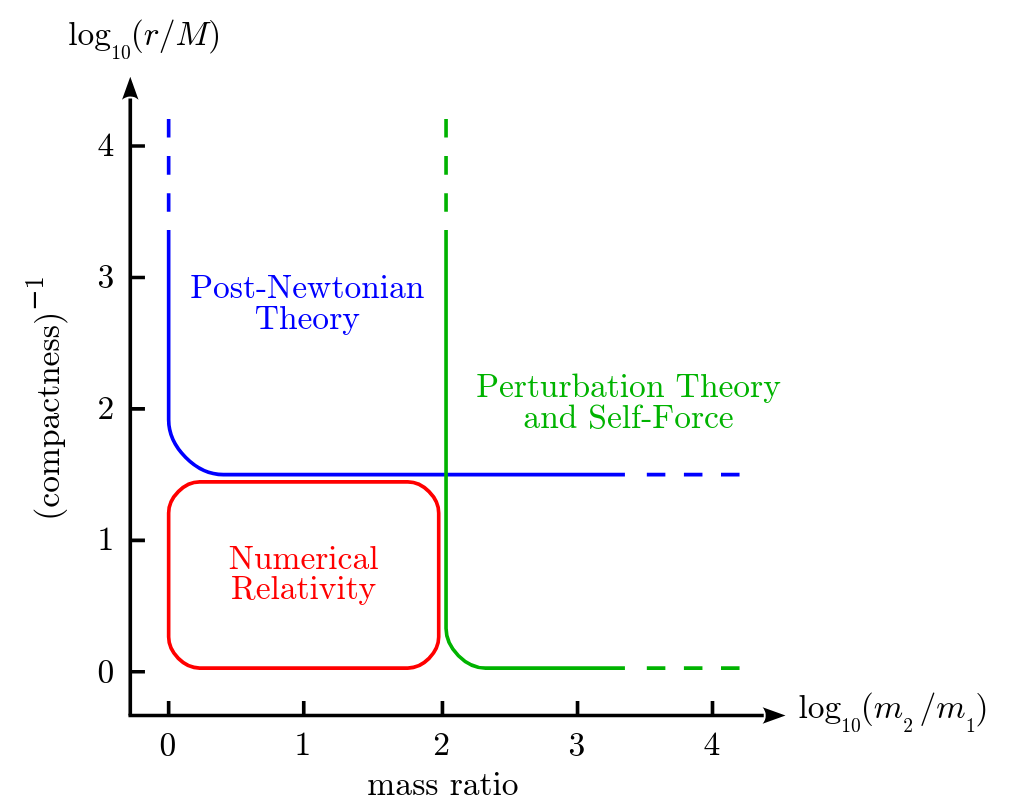
\includegraphics[width=0.8\textwidth]{theoretical_approaches_gw_waveforms.png}
    \caption[Overview of theoretical approaches to binary black holes]{Overview of the applicable regions for theoretical approaches to binary black holes. $m_1,m_2$ are the CO mass and MBH mass, $M = m_1 + m_2$ and $r$ is the separation. The figure is taken from \cite{Le_Tiec_2014}.}
    \label{fig:theoretical-approaches-gw-waveforms}
\end{figure}


\section{Black hole perturbation theory}
On fact that makes the EMRI event theoretically so appealing is the fact we can abuse the extreme ratio of MBH mass and CO mass $\frac{\Mbh}{\mu} \ll 1$ to shape the spacetime only considering the MBH, i.e. for example the Kerr black hole solution and then treat the CO as a perturbation of the metric that moves on this fixed background. This is known as black hole perturbation theory. One can then perform a perturbative expansion in the small parameter $\frac{\mu}{\Mbh}$ and we can understand the different orders as follow.
\begin{description}
    \item[Zeroth order] The CO moves along a geodesic of the background metric, i.e. the Kerr metric.
    \item[First order] The motion of the CO is adjusted by a small metric perturbation $h_{\mu\nu}$ and is accelerated by this effect which is called gravitational self-force. This gravitational self-force leads to a dissipation of energy that is related to the GW emission and a secular effect. This \emph{leading order} if GW emission in the case of a Kerr black hole and circular motion is known as the Teukolsky equation \cite{PhysRevX.4.041004}.
    \item[Second order] Subject to research and means taking second-order gravitational self-force effects into account.
\end{description}

\section{Post-Newtonian approximations}
In the case of Post-Newtonian (PN) approximations,  the perturbation that one considers applies to the case of large separations $r$ and therefore small values for $\frac{M}{r}$. This can only be applied up to a minimal separation where the perturbation ansatz fails.

\section{Numerical relativity}
We will ignore this approach here as it is not suitable in the case of EMRI events with $\frac{\mu}{M} \ll 1$.

\section{EMRI waveforms for data analysis}
To make EMRI signals available for mock data analysis we will later be using the python module \emph{FEW} \cite{Katz_2021,Chua_2021} (fast EMRI waveforms) which builds on the Augmented kludge waveform (AAK) introduced in \cite{PhysRevD.96.044005}. We will here give an overview of the approach to the generation of the EMRI waveforms. The main goal is to generate a waveform
\begin{equation}
    \label{eq:waveform-few}
    h(t) = h_+(t) + i h_\times(t),
\end{equation}
where $h_+(t)$ and $h_\times(t)$ are the two polarizations of the GW signal introduced in \fullref{chap:gravitational_waves}. At large distances (the resulting signal will be given in the solar barycenter frame (SSB)) the waveform takes the form
\begin{equation}
    \label{eq:waveform-few-expression}
    h(t) = \frac{\mu}{\dl} \sum_{lmkn} A_{lmkn}(t) S_{lmkn} (t, \theta) e^{im \phi} e^{-i \Phi_{mkn}(t)},
\end{equation}
where $\mu$ is the mass of the compact object, $\dl$ is the luminosity distance, $t$ is the arrival time of the signal in the barycenter frame, $\theta$ is the source-frame polar viewing angle, $\phi$ is the source-frame azimuthal viewing angle and $\{lmkn\}$ are the indices from the harmonic mode decomposition in the frequency domain. $\Phi_mkn \definedas m\Phi_\phi + k\Phi_\theta + n\Phi_r$ with the phases of each mode. $A_{lmkn} = -2 Z^\infty_{lmkn} \omega^{-2}_{mkn}$, where $\omega_{mkn} = m\Omega_\phi + k\Omega_\theta + n\Omega_r$ and $Z^\infty_{lmkn}$ is the Teukolsky mode amplitude far from the source. $\Omega_i$ are the frequencies of a Kerr geodes orbit. We just introduce all the notions here and refer to the original paper and the references therein for a detailed explanation. Overall, the waveform will be generated from the following parameters
\begin{itemize}\label{list:emri-parameters}
    \item $\Mbh$: mass of the MBH,
    \item $\mu$: mass of the compact object,
    \item $\dl$: luminosity distance,
    \item $\vartheta$: polar sky location angle in SSB frame,
    \item $\varphi$: azimuthal sky location angle in SSB frame,
    \item $a$: dimensionless spin of the MBH,
    \item $p_0$: initial semi-latus rectum,
    \item $e_0$: initial eccentricity,
    \item $x_{I,0} \definedas \cos (I_0)$: initial inclination angle $I_0$,
    \item $\vartheta_K$: polar angle of spin-angular momentum $\vec{S}$ of MBH,
    \item $\varphi_K$: azimuthal angle of spin-angular momentum $\vec{S}$ of MBH,
    \item $\Phi_{\theta,0}$: initial phase for $\theta$,
    \item $\Phi_{\phi,0}$: initial phase for $\phi$,
    \item $\Phi_{r,0}$: initial phase for $r$,
    \item $\tobs$: observation time,
    \item $\Delta t$: time step size for the waveform generation.
\end{itemize}
In \fullref{fig:FEW-waveform-generation} we see an overview of the EMRI waveform generation in the python module \emph{FEW}. Note, that we have already introduced observer-dependent parameters $(\vartheta, \varphi)$ that describe the sky localization of the EMRI event as seen from the SSB frame, which has nothing to do with the intrinsic evolution of the EMRI and boils down to a coordinate transformation after generating the waveform in the source frame.

\begin{figure}
    \centering
    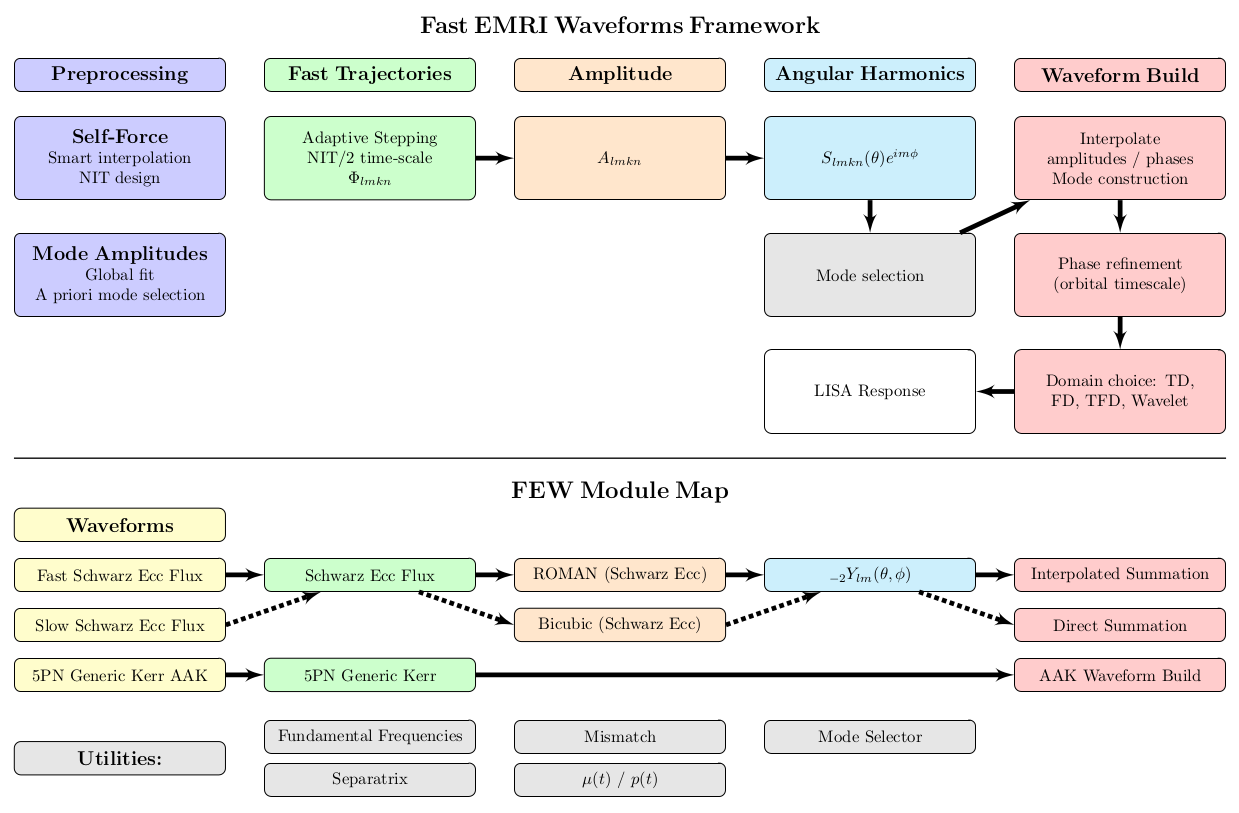
\includegraphics[width=0.8\textwidth]{FEW_waveform_generation.png}
    \caption[Overview of EMRI waveform generation via \emph{FEW}]{Overview of the EMRI waveform generation in the python module \emph{FEW} \cite{Katz_2021}. The figure is also taken from mentioned paper.}
    \label{fig:FEW-waveform-generation}
\end{figure}

\section{Redshift-mass degeneracy}
Let us note one important fact about the measurement of the mass of the MBH, because what we truly measure is the redshifted mass of the MBH or as derived in \cite[Equation 4.188]{10.1093/acprof:oso/9780198570745.001.0001} for the \emph{chirp mass}
\begin{equation}
    \label{eq:redshifted-mass}
    \Mbh^{\text{obs}} \equiv \Mz \definedas \Mbh (1+z),
\end{equation}
where $z$ is the redshift of the source and will be introduced in \fullref{ch:cosmology}.
